% Options for packages loaded elsewhere
\PassOptionsToPackage{unicode}{hyperref}
\PassOptionsToPackage{hyphens}{url}
%
\documentclass[
]{article}
\usepackage{amsmath,amssymb}
\usepackage{lmodern}
\usepackage{ifxetex,ifluatex}
\ifnum 0\ifxetex 1\fi\ifluatex 1\fi=0 % if pdftex
  \usepackage[T1]{fontenc}
  \usepackage[utf8]{inputenc}
  \usepackage{textcomp} % provide euro and other symbols
\else % if luatex or xetex
  \usepackage{unicode-math}
  \defaultfontfeatures{Scale=MatchLowercase}
  \defaultfontfeatures[\rmfamily]{Ligatures=TeX,Scale=1}
\fi
% Use upquote if available, for straight quotes in verbatim environments
\IfFileExists{upquote.sty}{\usepackage{upquote}}{}
\IfFileExists{microtype.sty}{% use microtype if available
  \usepackage[]{microtype}
  \UseMicrotypeSet[protrusion]{basicmath} % disable protrusion for tt fonts
}{}
\makeatletter
\@ifundefined{KOMAClassName}{% if non-KOMA class
  \IfFileExists{parskip.sty}{%
    \usepackage{parskip}
  }{% else
    \setlength{\parindent}{0pt}
    \setlength{\parskip}{6pt plus 2pt minus 1pt}}
}{% if KOMA class
  \KOMAoptions{parskip=half}}
\makeatother
\usepackage{xcolor}
\IfFileExists{xurl.sty}{\usepackage{xurl}}{} % add URL line breaks if available
\IfFileExists{bookmark.sty}{\usepackage{bookmark}}{\usepackage{hyperref}}
\hypersetup{
  pdftitle={CoDaCoRe Guide},
  pdfauthor={Elliott Gordon Rodriguez},
  hidelinks,
  pdfcreator={LaTeX via pandoc}}
\urlstyle{same} % disable monospaced font for URLs
\usepackage[margin=1in]{geometry}
\usepackage{color}
\usepackage{fancyvrb}
\newcommand{\VerbBar}{|}
\newcommand{\VERB}{\Verb[commandchars=\\\{\}]}
\DefineVerbatimEnvironment{Highlighting}{Verbatim}{commandchars=\\\{\}}
% Add ',fontsize=\small' for more characters per line
\usepackage{framed}
\definecolor{shadecolor}{RGB}{248,248,248}
\newenvironment{Shaded}{\begin{snugshade}}{\end{snugshade}}
\newcommand{\AlertTok}[1]{\textcolor[rgb]{0.94,0.16,0.16}{#1}}
\newcommand{\AnnotationTok}[1]{\textcolor[rgb]{0.56,0.35,0.01}{\textbf{\textit{#1}}}}
\newcommand{\AttributeTok}[1]{\textcolor[rgb]{0.77,0.63,0.00}{#1}}
\newcommand{\BaseNTok}[1]{\textcolor[rgb]{0.00,0.00,0.81}{#1}}
\newcommand{\BuiltInTok}[1]{#1}
\newcommand{\CharTok}[1]{\textcolor[rgb]{0.31,0.60,0.02}{#1}}
\newcommand{\CommentTok}[1]{\textcolor[rgb]{0.56,0.35,0.01}{\textit{#1}}}
\newcommand{\CommentVarTok}[1]{\textcolor[rgb]{0.56,0.35,0.01}{\textbf{\textit{#1}}}}
\newcommand{\ConstantTok}[1]{\textcolor[rgb]{0.00,0.00,0.00}{#1}}
\newcommand{\ControlFlowTok}[1]{\textcolor[rgb]{0.13,0.29,0.53}{\textbf{#1}}}
\newcommand{\DataTypeTok}[1]{\textcolor[rgb]{0.13,0.29,0.53}{#1}}
\newcommand{\DecValTok}[1]{\textcolor[rgb]{0.00,0.00,0.81}{#1}}
\newcommand{\DocumentationTok}[1]{\textcolor[rgb]{0.56,0.35,0.01}{\textbf{\textit{#1}}}}
\newcommand{\ErrorTok}[1]{\textcolor[rgb]{0.64,0.00,0.00}{\textbf{#1}}}
\newcommand{\ExtensionTok}[1]{#1}
\newcommand{\FloatTok}[1]{\textcolor[rgb]{0.00,0.00,0.81}{#1}}
\newcommand{\FunctionTok}[1]{\textcolor[rgb]{0.00,0.00,0.00}{#1}}
\newcommand{\ImportTok}[1]{#1}
\newcommand{\InformationTok}[1]{\textcolor[rgb]{0.56,0.35,0.01}{\textbf{\textit{#1}}}}
\newcommand{\KeywordTok}[1]{\textcolor[rgb]{0.13,0.29,0.53}{\textbf{#1}}}
\newcommand{\NormalTok}[1]{#1}
\newcommand{\OperatorTok}[1]{\textcolor[rgb]{0.81,0.36,0.00}{\textbf{#1}}}
\newcommand{\OtherTok}[1]{\textcolor[rgb]{0.56,0.35,0.01}{#1}}
\newcommand{\PreprocessorTok}[1]{\textcolor[rgb]{0.56,0.35,0.01}{\textit{#1}}}
\newcommand{\RegionMarkerTok}[1]{#1}
\newcommand{\SpecialCharTok}[1]{\textcolor[rgb]{0.00,0.00,0.00}{#1}}
\newcommand{\SpecialStringTok}[1]{\textcolor[rgb]{0.31,0.60,0.02}{#1}}
\newcommand{\StringTok}[1]{\textcolor[rgb]{0.31,0.60,0.02}{#1}}
\newcommand{\VariableTok}[1]{\textcolor[rgb]{0.00,0.00,0.00}{#1}}
\newcommand{\VerbatimStringTok}[1]{\textcolor[rgb]{0.31,0.60,0.02}{#1}}
\newcommand{\WarningTok}[1]{\textcolor[rgb]{0.56,0.35,0.01}{\textbf{\textit{#1}}}}
\usepackage{graphicx}
\makeatletter
\def\maxwidth{\ifdim\Gin@nat@width>\linewidth\linewidth\else\Gin@nat@width\fi}
\def\maxheight{\ifdim\Gin@nat@height>\textheight\textheight\else\Gin@nat@height\fi}
\makeatother
% Scale images if necessary, so that they will not overflow the page
% margins by default, and it is still possible to overwrite the defaults
% using explicit options in \includegraphics[width, height, ...]{}
\setkeys{Gin}{width=\maxwidth,height=\maxheight,keepaspectratio}
% Set default figure placement to htbp
\makeatletter
\def\fps@figure{htbp}
\makeatother
\setlength{\emergencystretch}{3em} % prevent overfull lines
\providecommand{\tightlist}{%
  \setlength{\itemsep}{0pt}\setlength{\parskip}{0pt}}
\setcounter{secnumdepth}{-\maxdimen} % remove section numbering
\ifluatex
  \usepackage{selnolig}  % disable illegal ligatures
\fi

\title{CoDaCoRe Guide}
\author{Elliott Gordon Rodriguez\footnote{\href{mailto:eg2912@columbia.edu}{\nolinkurl{eg2912@columbia.edu}}}}
\date{2022-02-26}

\begin{document}
\maketitle

\hypertarget{installation}{%
\section{Installation}\label{installation}}

You can install \texttt{codacore} by running:

\begin{Shaded}
\begin{Highlighting}[]
\FunctionTok{install.packages}\NormalTok{(}\StringTok{"codacore"}\NormalTok{)}
\end{Highlighting}
\end{Shaded}

You may instead install the
\href{https://github.com/egr95/R-codacore}{development version} directly
from Github, using the
\href{https://www.r-project.org/nosvn/pandoc/devtools.html}{devtools
package}.

\begin{Shaded}
\begin{Highlighting}[]
\NormalTok{devtools}\SpecialCharTok{::}\FunctionTok{install\_github}\NormalTok{(}\StringTok{"egr95/R{-}codacore"}\NormalTok{, }\AttributeTok{ref=}\StringTok{"main"}\NormalTok{)}
\end{Highlighting}
\end{Shaded}

Note that CoDaCoRe requires a working installation of
\href{https://tensorflow.rstudio.com/}{TensorFlow}. If you do not have
Tensorflow previously installed, when you run \texttt{codacore()} for
the first time you will likely encounter an error message of the form:

\begin{Shaded}
\begin{Highlighting}[]
\SpecialCharTok{\textgreater{}} \FunctionTok{codacore}\NormalTok{(x, y)}

\NormalTok{ERROR}\SpecialCharTok{:}\NormalTok{ Could not find a version that satisfies the requirement tensorflow}
\NormalTok{ERROR}\SpecialCharTok{:}\NormalTok{ No matching distribution found }\ControlFlowTok{for}\NormalTok{ tensorflow}
\NormalTok{Error}\SpecialCharTok{:}\NormalTok{ Installation of TensorFlow not found.}

\NormalTok{Python environments searched }\ControlFlowTok{for} \StringTok{\textquotesingle{}tensorflow\textquotesingle{}}\NormalTok{ package}\SpecialCharTok{:}
 \ErrorTok{/}\NormalTok{moto}\SpecialCharTok{/}\NormalTok{stats}\SpecialCharTok{/}\NormalTok{users}\SpecialCharTok{/}\NormalTok{eg2912}\SpecialCharTok{/}\NormalTok{miniconda3}\SpecialCharTok{/}\NormalTok{envs}\SpecialCharTok{/}\NormalTok{r}\SpecialCharTok{{-}}\NormalTok{test}\SpecialCharTok{/}\NormalTok{bin}\SpecialCharTok{/}\NormalTok{python3}\FloatTok{.9}
 \SpecialCharTok{/}\NormalTok{usr}\SpecialCharTok{/}\NormalTok{bin}\SpecialCharTok{/}\NormalTok{python2}\FloatTok{.7}

\NormalTok{You can install TensorFlow using the }\FunctionTok{install\_tensorflow}\NormalTok{() function.}
\end{Highlighting}
\end{Shaded}

This can be fixed simply by
\href{https://tensorflow.rstudio.com/installation/}{installing
tensorflow}, as follows:

\begin{Shaded}
\begin{Highlighting}[]
\FunctionTok{install.packages}\NormalTok{(}\StringTok{"tensorflow"}\NormalTok{)}
\FunctionTok{library}\NormalTok{(}\StringTok{"tensorflow"}\NormalTok{)}
\FunctionTok{install\_tensorflow}\NormalTok{()}

\FunctionTok{install.packages}\NormalTok{(}\StringTok{"keras"}\NormalTok{)}
\FunctionTok{library}\NormalTok{(}\StringTok{"keras"}\NormalTok{)}
\FunctionTok{install\_keras}\NormalTok{()}
\end{Highlighting}
\end{Shaded}

Note also that you may have to restart your R session between
installation of \texttt{codacore}, \texttt{tensorflow}, and
\texttt{keras}.

\hypertarget{summary-of-method}{%
\section{Summary of method}\label{summary-of-method}}

CoDaCoRe is an algorithm to identify predictive log-ratio biomarkers in
high-throughput sequencing data. Let \(x\) denote HTS input (e.g.,
\(x_{i,j}\) denotes the abundance of the \(j\)th bacteria in the \(i\)th
subject), and let \(y\) denote the outcome of interest (e.g., \(y_i\) is
equal to 0 or 1 depending on whether the \(i\)th subject belonged to the
case or the control group). Given a set of \((x_i, y_i)\) pairs,
CoDaCoRe identifies predictive biomarkers of the form: \[
B(x_i; J^+, J^-) = \log \left( \frac{\sum_{j \in J^+} x_{i,j}}{\sum_{j \in J^-} x_{i,j}} \right),
\] that are maximally associated with the response variable \(y_i\). In
other words, CoDaCoRe identifies a numerator set \(J^+\) and a
denominator set \(J^-\), such that their log-ratio is most predictive of
the response variable. By default, CoDaCoRe uses \emph{balances}, which
are defined as the log-ratio of \emph{geometric means} (as opposed to
summations): \[
B(x_i; J^+, J^-) = \log \left( \frac{(\prod_{j \in J^+} x_{i,j})^{|J^+|}}{(\prod_{j \in J^-} x_{i,j})^{|J^-|}} \right).
\]

For an introduction to balances, we refer the reader to the
\href{https://journals.asm.org/doi/abs/10.1128/msystems.00053-18}{selbal
paper}, and for a more detailed treatment of CoDaCoRe and other
log-ratio methodology, we refer the reader to the
\href{https://doi.org/10.1093/bioinformatics/btab645}{codacore paper}
and \href{https://arxiv.org/abs/2104.07266}{this paper}.

\hypertarget{training-the-model}{%
\section{Training the model}\label{training-the-model}}

We assume a working installation of \texttt{codacore}
(\href{https://github.com/egr95/R-codacore/blob/main/README.md}{link}).

\begin{Shaded}
\begin{Highlighting}[]
\FunctionTok{library}\NormalTok{(}\StringTok{"codacore"}\NormalTok{)}
\FunctionTok{help}\NormalTok{(codacore)}
\end{Highlighting}
\end{Shaded}

In this tutorial, we will showcase \texttt{codacore} using three
datasets that were also analyzed by the authors of \texttt{selbal}
\href{https://journals.asm.org/doi/abs/10.1128/msystems.00053-18}{(Rivera-Pinto
et al., 2018)}. First, we consider the Crohn's disease data from
\href{http://dx.doi.org/10.1016/j.chom.2014.02.005}{(Gevers et al.,
2014)}.

\begin{Shaded}
\begin{Highlighting}[]
\FunctionTok{data}\NormalTok{(}\StringTok{"Crohn"}\NormalTok{)}
\NormalTok{x }\OtherTok{\textless{}{-}}\NormalTok{ Crohn[, }\SpecialCharTok{{-}}\FunctionTok{ncol}\NormalTok{(Crohn)]}
\NormalTok{y }\OtherTok{\textless{}{-}}\NormalTok{ Crohn[, }\FunctionTok{ncol}\NormalTok{(Crohn)]}
\end{Highlighting}
\end{Shaded}

Our goal is to identify ratio-based biomarkers that are predictive of
disease status. Our input variable consists of the abundance of 48
microbial species in 975 samples.

\begin{Shaded}
\begin{Highlighting}[]
\FunctionTok{dim}\NormalTok{(x)}
\CommentTok{\#\textgreater{} [1] 975  48}
\end{Highlighting}
\end{Shaded}

The output variable is a binary indicator (CD stands for Chron's
disease).

\begin{Shaded}
\begin{Highlighting}[]
\FunctionTok{table}\NormalTok{(y)}
\CommentTok{\#\textgreater{} y}
\CommentTok{\#\textgreater{}  CD  no }
\CommentTok{\#\textgreater{} 662 313}
\end{Highlighting}
\end{Shaded}

Prior to fitting CoDaCoRe, we must impute any zeros in our input
variable (a standard pre-processing step for ratio-based methods).

\begin{Shaded}
\begin{Highlighting}[]
\NormalTok{x }\OtherTok{\textless{}{-}}\NormalTok{ x }\SpecialCharTok{+} \DecValTok{1}
\end{Highlighting}
\end{Shaded}

Next, we split our data into a training and a test set (to keep things
simple we do this naively at random, though in practice one might
consider stratified sampling and class rebalancing).

\begin{Shaded}
\begin{Highlighting}[]
\CommentTok{\# For reproducibility, we set a random}
\CommentTok{\# seed (including in TensorFlow, used}
\CommentTok{\# by codacore)}
\FunctionTok{set.seed}\NormalTok{(}\DecValTok{0}\NormalTok{)}
\FunctionTok{library}\NormalTok{(tensorflow)}
\NormalTok{tf}\SpecialCharTok{$}\NormalTok{random}\SpecialCharTok{$}\FunctionTok{set\_seed}\NormalTok{(}\DecValTok{0}\NormalTok{)}
\NormalTok{trainIndex }\OtherTok{\textless{}{-}} \FunctionTok{sample}\NormalTok{(}\DecValTok{1}\SpecialCharTok{:}\FunctionTok{nrow}\NormalTok{(x), }\FloatTok{0.8} \SpecialCharTok{*} \FunctionTok{nrow}\NormalTok{(x))}
\NormalTok{xTrain }\OtherTok{\textless{}{-}}\NormalTok{ x[trainIndex, ]}
\NormalTok{yTrain }\OtherTok{\textless{}{-}}\NormalTok{ y[trainIndex]}
\end{Highlighting}
\end{Shaded}

We are ready to fit CoDaCoRe. We stick to the default parameters for
now. Notice the fast runtime (as compared to, for example,
\texttt{selbal.cv}).

\begin{Shaded}
\begin{Highlighting}[]
\NormalTok{model }\OtherTok{\textless{}{-}} \FunctionTok{codacore}\NormalTok{(}
\NormalTok{  xTrain,}
\NormalTok{  yTrain,}
  \AttributeTok{logRatioType =} \StringTok{\textquotesingle{}balances\textquotesingle{}}\NormalTok{, }\CommentTok{\# can also use \textquotesingle{}amalgamations\textquotesingle{}}
  \AttributeTok{lambda =} \DecValTok{1}                 \CommentTok{\# regularization parameter (1 corresponds to "1SE rule")}
\NormalTok{)}
\end{Highlighting}
\end{Shaded}

\hypertarget{visualizing-results}{%
\section{Visualizing results}\label{visualizing-results}}

Next we can check the learned output of the model: what inputs were
included in the learned log-ratios, how strongly associated they are to
the response, and how well they classified the data.

\begin{Shaded}
\begin{Highlighting}[]
\FunctionTok{print}\NormalTok{(model)}
\CommentTok{\#\textgreater{} }
\CommentTok{\#\textgreater{} Number of log{-}ratios found: 2}
\CommentTok{\#\textgreater{} ***}
\CommentTok{\#\textgreater{} Log{-}ratio rank 1}
\CommentTok{\#\textgreater{} Numerator: g\_\_Roseburia o\_\_Clostridiales\_g\_\_}
\CommentTok{\#\textgreater{} Denominator: g\_\_Dialister g\_\_Aggregatibacter}
\CommentTok{\#\textgreater{} AUC: 0.7567907}
\CommentTok{\#\textgreater{} Slope: 0.3939618}
\CommentTok{\#\textgreater{} ***}
\CommentTok{\#\textgreater{} Log{-}ratio rank 2}
\CommentTok{\#\textgreater{} Numerator: g\_\_Parabacteroides f\_\_Peptostreptococcaceae\_g\_\_ g\_\_Bacteroides g\_\_Faecalibacterium g\_\_Roseburia g\_\_Lachnospira o\_\_Clostridiales\_g\_\_ f\_\_Rikenellaceae\_g\_\_}
\CommentTok{\#\textgreater{} Denominator: g\_\_Eggerthella g\_\_Dialister g\_\_Streptococcus g\_\_Aggregatibacter}
\CommentTok{\#\textgreater{} AUC: 0.778969}
\CommentTok{\#\textgreater{} Slope: 0.3002488}
\end{Highlighting}
\end{Shaded}

The most predictive ratio identified by CoDaCoRe is Roseburia /
Dialister, which can be visualized with the \texttt{plot} function.

\begin{Shaded}
\begin{Highlighting}[]
\FunctionTok{plot}\NormalTok{(model)}
\end{Highlighting}
\end{Shaded}

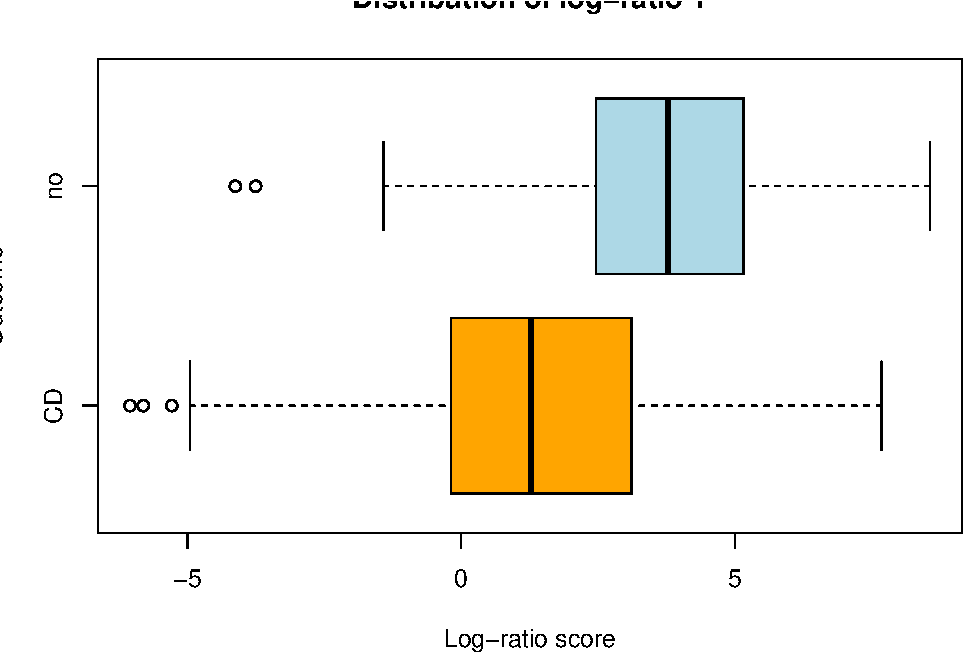
\includegraphics{guide_files/figure-latex/unnamed-chunk-10-1.pdf}

Note that CoDaCoRe is an ensemble model, where multiple log-ratios are
learned sequentially in decreasing order of importance (with automatic
stopping whenever no additional log-ratio improved the loss function
during training). We can visualize the performance of this ensembling
procedure by ``stacking'' the respective ROC curves.

\begin{Shaded}
\begin{Highlighting}[]
\FunctionTok{plotROC}\NormalTok{(model)}
\end{Highlighting}
\end{Shaded}

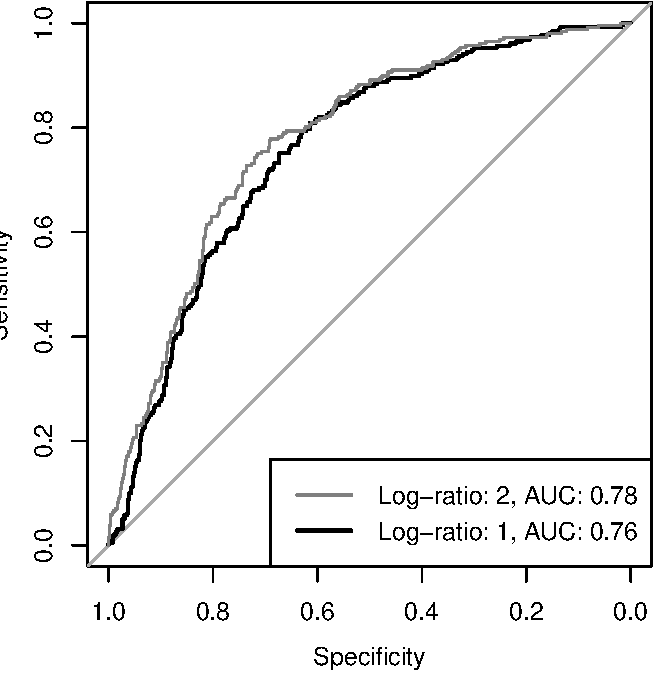
\includegraphics{guide_files/figure-latex/unnamed-chunk-11-1.pdf}

\hypertarget{predicting-on-new-data}{%
\section{Predicting on new data}\label{predicting-on-new-data}}

We can also use our trained model to classify new samples.

\begin{Shaded}
\begin{Highlighting}[]
\NormalTok{xTest }\OtherTok{\textless{}{-}}\NormalTok{ x[}\SpecialCharTok{{-}}\NormalTok{trainIndex, ]}
\NormalTok{yTest }\OtherTok{\textless{}{-}}\NormalTok{ y[}\SpecialCharTok{{-}}\NormalTok{trainIndex]}
\NormalTok{yHat }\OtherTok{\textless{}{-}} \FunctionTok{predict}\NormalTok{(model, xTest, }\AttributeTok{logits =}\NormalTok{ F)}
\FunctionTok{cat}\NormalTok{(}\StringTok{"Test set AUC ="}\NormalTok{, pROC}\SpecialCharTok{::}\FunctionTok{auc}\NormalTok{(pROC}\SpecialCharTok{::}\FunctionTok{roc}\NormalTok{(yTest,}
\NormalTok{    yHat, }\AttributeTok{quiet =}\NormalTok{ T)))}
\CommentTok{\#\textgreater{} Test set AUC = 0.80537}
\CommentTok{\# Convert probabilities into a binary}
\CommentTok{\# class}
\NormalTok{failure }\OtherTok{\textless{}{-}}\NormalTok{ yHat }\SpecialCharTok{\textless{}} \FloatTok{0.5}
\NormalTok{success }\OtherTok{\textless{}{-}}\NormalTok{ yHat }\SpecialCharTok{\textgreater{}=} \FloatTok{0.5}
\NormalTok{yHat[failure] }\OtherTok{\textless{}{-}} \FunctionTok{levels}\NormalTok{(y)[}\DecValTok{1}\NormalTok{]}
\NormalTok{yHat[success] }\OtherTok{\textless{}{-}} \FunctionTok{levels}\NormalTok{(y)[}\DecValTok{2}\NormalTok{]}
\FunctionTok{cat}\NormalTok{(}\StringTok{"Classification accuracy on test set ="}\NormalTok{,}
    \FunctionTok{round}\NormalTok{(}\FunctionTok{mean}\NormalTok{(yHat }\SpecialCharTok{==}\NormalTok{ yTest), }\DecValTok{2}\NormalTok{))}
\CommentTok{\#\textgreater{} Classification accuracy on test set = 0.73}
\end{Highlighting}
\end{Shaded}

Note our \texttt{predict} function can be restricted to only use the top
\emph{k} log-ratios in the model for prediction. For example, the
following will compute the AUC of a 1-log-ratio model, using only the
top log-ratio.

\begin{Shaded}
\begin{Highlighting}[]
\NormalTok{yHat }\OtherTok{\textless{}{-}} \FunctionTok{predict}\NormalTok{(model, xTest, }\AttributeTok{logits =}\NormalTok{ F,}
    \AttributeTok{numLogRatios =} \DecValTok{1}\NormalTok{)}
\FunctionTok{cat}\NormalTok{(}\StringTok{"Test set AUC ="}\NormalTok{, pROC}\SpecialCharTok{::}\FunctionTok{auc}\NormalTok{(pROC}\SpecialCharTok{::}\FunctionTok{roc}\NormalTok{(yTest,}
\NormalTok{    yHat, }\AttributeTok{quiet =}\NormalTok{ T)))}
\CommentTok{\#\textgreater{} Test set AUC = 0.7859712}
\end{Highlighting}
\end{Shaded}

Other useful functions include:

\begin{Shaded}
\begin{Highlighting}[]
\FunctionTok{getNumeratorParts}\NormalTok{(model, }\DecValTok{1}\NormalTok{)}
\FunctionTok{getDenominatorParts}\NormalTok{(model, }\DecValTok{1}\NormalTok{)}
\FunctionTok{getLogRatios}\NormalTok{(model, xTest)}
\FunctionTok{getNumLogRatios}\NormalTok{(model)}
\FunctionTok{getTidyTable}\NormalTok{(model)}
\FunctionTok{getSlopes}\NormalTok{(model)}
\end{Highlighting}
\end{Shaded}

\hypertarget{controlling-overlap-between-log-ratios}{%
\section{Controlling overlap between
log-ratios}\label{controlling-overlap-between-log-ratios}}

By default, CoDaCoRe allows for ``overlapping log-ratios'', in other
words, an input variable that is included in the first log-ratio may
well be included in a second or third log-ratio provided it is
sufficiently predictive. However, the user may choose to restrict each
successive log-ratio to be constructed from a mutually exclusive set of
input variables (e.g., to obtain \emph{orthogonal balances}, in the
Aitchison sense). This can be specified with the parameter
\texttt{overlap}. In our example, note how \texttt{g\_\_Dialister} is no
longer repeated.

\begin{Shaded}
\begin{Highlighting}[]
\NormalTok{model }\OtherTok{\textless{}{-}} \FunctionTok{codacore}\NormalTok{(xTrain, yTrain, }\AttributeTok{overlap =}\NormalTok{ F)}
\FunctionTok{print}\NormalTok{(model)}
\CommentTok{\#\textgreater{} }
\CommentTok{\#\textgreater{} Number of log{-}ratios found: 2}
\CommentTok{\#\textgreater{} ***}
\CommentTok{\#\textgreater{} Log{-}ratio rank 1}
\CommentTok{\#\textgreater{} Numerator: g\_\_Roseburia o\_\_Clostridiales\_g\_\_}
\CommentTok{\#\textgreater{} Denominator: g\_\_Dialister g\_\_Aggregatibacter}
\CommentTok{\#\textgreater{} AUC: 0.7567907}
\CommentTok{\#\textgreater{} Slope: 0.3939618}
\CommentTok{\#\textgreater{} ***}
\CommentTok{\#\textgreater{} Log{-}ratio rank 2}
\CommentTok{\#\textgreater{} Numerator: g\_\_Parabacteroides f\_\_Peptostreptococcaceae\_g\_\_ g\_\_Bacteroides g\_\_Faecalibacterium g\_\_Lachnospira f\_\_Rikenellaceae\_g\_\_}
\CommentTok{\#\textgreater{} Denominator: g\_\_Eggerthella f\_\_Enterobacteriaceae\_g\_\_}
\CommentTok{\#\textgreater{} AUC: 0.7712166}
\CommentTok{\#\textgreater{} Slope: 0.1858207}
\end{Highlighting}
\end{Shaded}

\hypertarget{using-amalgamations-summed-log-ratios}{%
\section{Using amalgamations
(summed-log-ratios)}\label{using-amalgamations-summed-log-ratios}}

CoDaCoRe can be used to learn log-ratios between both geometric means
(known as ``balances'' or ``isometric-log-ratio'') or summations (known
as ``amalgamations'' or ``summed-log-ratio''), depending on the goals of
the user. This can be specified with the parameter
\texttt{logRatioType}.

\begin{Shaded}
\begin{Highlighting}[]
\NormalTok{model }\OtherTok{\textless{}{-}} \FunctionTok{codacore}\NormalTok{(xTrain, yTrain, }\AttributeTok{logRatioType =} \StringTok{"amalgamations"}\NormalTok{)}
\FunctionTok{print}\NormalTok{(model)}
\CommentTok{\#\textgreater{} }
\CommentTok{\#\textgreater{} Number of log{-}ratios found: 1}
\CommentTok{\#\textgreater{} ***}
\CommentTok{\#\textgreater{} Log{-}ratio rank 1}
\CommentTok{\#\textgreater{} Numerator: g\_\_Parabacteroides g\_\_Bacteroides g\_\_Faecalibacterium o\_\_Clostridiales\_g\_\_}
\CommentTok{\#\textgreater{} Denominator: g\_\_Haemophilus g\_\_Blautia f\_\_Enterobacteriaceae\_g\_\_ g\_\_Dialister g\_\_Streptococcus g\_\_Fusobacterium}
\CommentTok{\#\textgreater{} AUC: 0.7104552}
\CommentTok{\#\textgreater{} Slope: 0.4062366}
\end{Highlighting}
\end{Shaded}

Note that amalgamations/summed-log-ratios are less sensitive to
covariates that are small in magnitude (e.g., rare microbes), which can
hinder their predictive strength for datasets where small covariates are
important. On the other hand, summed-log-ratios have a different
interpretation than isometric-log-ratios and may therefore be
preferrable in some applications (e.g., when the ``summed'' effect of an
aggregated sub-population is the object of interest). In our Crohn's
disease data, the rare species Roseburia gets picked up by the
isometric-log-ratio, but not by the summed-log-ratio, which is more
sensitive to more common bacteria species such as Faecalibacterium.

\hypertarget{continuous-outcomes}{%
\section{Continuous outcomes}\label{continuous-outcomes}}

We consider the HIV data from
\href{http://dx.doi.org/10.1016/j.ebiom.2016.01.032}{(Noguera-Julian et
al., 2016)}. The goal here is to construct a log-ratio of the microbial
abundances that is predictive of the inflammation marker ``sCD14'', a
continuous response variable. CoDaCoRe can be applied much in the same
way, except the loss function changes from binary cross-entropy to
mean-squared-error. This change will happen automatically based on the
values inputted as \texttt{y} (although it can also be overriden
manually via the \texttt{objective} parameter, for example, if the user
wanted to fit a binary response using the mean-squared-error, they could
specify
\texttt{objective\ =\ \textquotesingle{}regression\textquotesingle{}}).

\begin{Shaded}
\begin{Highlighting}[]
\FunctionTok{data}\NormalTok{(}\StringTok{"sCD14"}\NormalTok{)}
\NormalTok{x }\OtherTok{\textless{}{-}}\NormalTok{ sCD14[, }\SpecialCharTok{{-}}\FunctionTok{ncol}\NormalTok{(sCD14)]}
\NormalTok{y }\OtherTok{\textless{}{-}}\NormalTok{ sCD14[, }\FunctionTok{ncol}\NormalTok{(sCD14)]}

\CommentTok{\# Replace zeros as before}
\NormalTok{x }\OtherTok{\textless{}{-}}\NormalTok{ x }\SpecialCharTok{+} \DecValTok{1}

\CommentTok{\# Split the data}
\NormalTok{trainIndex }\OtherTok{\textless{}{-}} \FunctionTok{sample}\NormalTok{(}\DecValTok{1}\SpecialCharTok{:}\FunctionTok{nrow}\NormalTok{(x), }\FloatTok{0.8} \SpecialCharTok{*} \FunctionTok{nrow}\NormalTok{(x))}
\NormalTok{xTrain }\OtherTok{\textless{}{-}}\NormalTok{ x[trainIndex, ]}
\NormalTok{yTrain }\OtherTok{\textless{}{-}}\NormalTok{ y[trainIndex]}

\CommentTok{\# Fit codacore and inspect results}
\NormalTok{model }\OtherTok{\textless{}{-}} \FunctionTok{codacore}\NormalTok{(xTrain, yTrain)}
\FunctionTok{print}\NormalTok{(model)}
\CommentTok{\#\textgreater{} }
\CommentTok{\#\textgreater{} Number of log{-}ratios found: 1}
\CommentTok{\#\textgreater{} ***}
\CommentTok{\#\textgreater{} Log{-}ratio rank 1}
\CommentTok{\#\textgreater{} Numerator: g\_Subdoligranulum}
\CommentTok{\#\textgreater{} Denominator: g\_Bifidobacterium}
\CommentTok{\#\textgreater{} R squared: 0.1438051}
\CommentTok{\#\textgreater{} Slope: 611.0956}
\FunctionTok{plot}\NormalTok{(model)}
\end{Highlighting}
\end{Shaded}

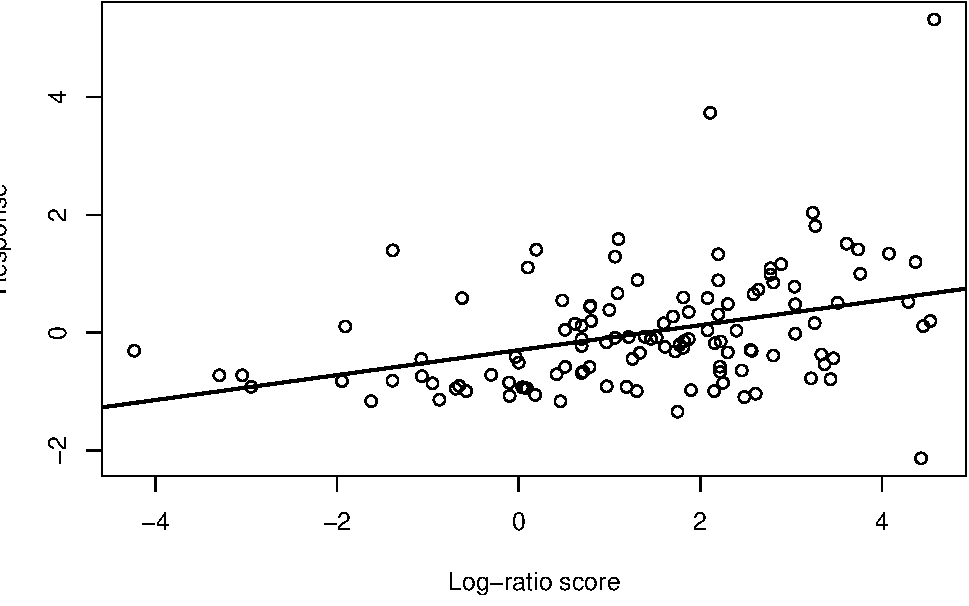
\includegraphics{guide_files/figure-latex/unnamed-chunk-17-1.pdf}

\hypertarget{tuning-the-regularization-parameter-lambda}{%
\section{Tuning the regularization parameter
lambda}\label{tuning-the-regularization-parameter-lambda}}

The parameter \texttt{lambda} controls the regularization strength of
CoDaCoRe. In particular, \texttt{lambda\ =\ 1} (the default value)
corresponds to applying the 1-standard-error rule in the discretization
step of the log-ratio (details in
\href{https://www.biorxiv.org/content/10.1101/2021.02.11.430695v2.full.pdf}{Section
3.3}). This is typically a good choice, leading to models that are both
sparse and predictive. Sparser models can be achieved by higher values
of \texttt{lambda}, for example, \texttt{lambda\ =\ 2} corresponds to
applying a ``2-standard-error'' rule. On the other hand, smaller values
of lambda result in less sparse, but typically most predictive, models.
In particular, \texttt{lambda\ =\ 0} corresponds to a ``0 standard-error
rule'', in other words choosing the log-ratio that minimizes
cross-validation score. Such a choice can be good when we seek a
maximally predictive model, but care less about sparsity.

\begin{Shaded}
\begin{Highlighting}[]
\NormalTok{model }\OtherTok{\textless{}{-}} \FunctionTok{codacore}\NormalTok{(xTrain, yTrain, }\AttributeTok{lambda =} \DecValTok{0}\NormalTok{)}
\FunctionTok{print}\NormalTok{(model)}
\CommentTok{\#\textgreater{} }
\CommentTok{\#\textgreater{} Number of log{-}ratios found: 3}
\CommentTok{\#\textgreater{} ***}
\CommentTok{\#\textgreater{} Log{-}ratio rank 1}
\CommentTok{\#\textgreater{} Numerator: g\_Subdoligranulum g\_Dialister g\_Paraprevotella f\_Defluviitaleaceae\_g\_Incertae\_Sedis}
\CommentTok{\#\textgreater{} Denominator: f\_Lachnospiraceae\_g\_unclassified g\_Succinivibrio g\_Parabacteroides g\_Lachnospira g\_Coprococcus g\_Catenibacterium g\_Roseburia g\_Megasphaera g\_Mitsuokella g\_Sutterella g\_Bifidobacterium g\_Streptococcus f\_Erysipelotrichaceae\_g\_unclassified f\_Porphyromonadaceae\_g\_unclassified g\_Collinsella}
\CommentTok{\#\textgreater{} R squared: 0.319985}
\CommentTok{\#\textgreater{} Slope: 2040.222}
\CommentTok{\#\textgreater{} ***}
\CommentTok{\#\textgreater{} Log{-}ratio rank 2}
\CommentTok{\#\textgreater{} Numerator: g\_Faecalibacterium g\_Bacteroides g\_Alloprevotella g\_Subdoligranulum g\_Clostridium\_sensu\_stricto\_1 g\_Escherichia{-}Shigella f\_Defluviitaleaceae\_g\_Incertae\_Sedis}
\CommentTok{\#\textgreater{} Denominator: f\_Lachnospiraceae\_g\_unclassified g\_Lachnospira g\_Barnesiella g\_Catenibacterium g\_Megasphaera g\_Mitsuokella g\_Sutterella g\_Bifidobacterium g\_Collinsella}
\CommentTok{\#\textgreater{} R squared: 0.3852063}
\CommentTok{\#\textgreater{} Slope: 816.7075}
\CommentTok{\#\textgreater{} ***}
\CommentTok{\#\textgreater{} Log{-}ratio rank 3}
\CommentTok{\#\textgreater{} Numerator: g\_Alloprevotella}
\CommentTok{\#\textgreater{} Denominator: g\_Bifidobacterium}
\CommentTok{\#\textgreater{} R squared: 0.390754}
\CommentTok{\#\textgreater{} Slope: 66.46405}
\end{Highlighting}
\end{Shaded}

Notice the increased R-squared score relative to the previous model (at
the expense of sparsity).

\hypertarget{when-no-predictive-log-ratios-are-found}{%
\subsection{When no predictive log-ratios are
found}\label{when-no-predictive-log-ratios-are-found}}

On some datasets, CoDaCoRe may have trouble finding \emph{any}
predictive log-ratios. If none are found, this is typically a sign that
the signal in the data is weak. In this case, the analyst may choose to
reduce the value of \texttt{lambda} (for example, to
\texttt{lambda\ =\ 0}), in order to allow our algorithm to search more
aggressively for predictive log-ratios. Doing so will often allow the
algorithm to identify at least one predictive log-ratio, at the risk of
overfitting the training data. Additional care must be taken in
validating such log-ratios on held-out data.

\hypertarget{covariate-adjustment}{%
\section{Covariate adjustment}\label{covariate-adjustment}}

Many applications require accounting for potential confounder variables
as well as our ratio-based biomarkers. As an example, we consider a
second HIV dataset from
\href{http://dx.doi.org/10.1016/j.ebiom.2016.01.032}{(Noguera-Julian et
al.~2016)}. The goal is to find a microbial signature for HIV status,
i.e., a log-ratio that can discriminate between HIV-positive and
HIV-negative individuals. However, we have an additional confounder
variable, MSM (Men who have Sex with Men). In the context of CoDaCoRe,
there are multiple approaches that can be used to adjust for covariates.

\hypertarget{incremental-fit}{%
\subsection{Incremental fit}\label{incremental-fit}}

Given the \emph{stagewise-additive} (i.e., ensemble) nature of CoDaCoRe,
whereby each successive log-ratio is fitted on the residual of the
previous iteration, a very natural approach is to fit the covariates
\emph{a priori} and then fit CoDaCoRe on the residual. In other words,
we would start by regressing HIV status on MSM, ``partialling out'' this
covariate, and then fit CoDaCoRe on the residual from this model. This
can be implemented easily by means of the \texttt{offset} parameter.

\begin{Shaded}
\begin{Highlighting}[]
\FunctionTok{data}\NormalTok{(}\StringTok{"HIV"}\NormalTok{)}
\NormalTok{x }\OtherTok{\textless{}{-}}\NormalTok{ HIV[, }\DecValTok{1}\SpecialCharTok{:}\NormalTok{(}\FunctionTok{ncol}\NormalTok{(HIV) }\SpecialCharTok{{-}} \DecValTok{2}\NormalTok{)]}
\NormalTok{z }\OtherTok{\textless{}{-}}\NormalTok{ HIV[, }\StringTok{"MSM"}\NormalTok{]}
\NormalTok{y }\OtherTok{\textless{}{-}}\NormalTok{ HIV}\SpecialCharTok{$}\NormalTok{HIV\_Status}

\CommentTok{\# Replace zeros as before}
\NormalTok{x }\OtherTok{\textless{}{-}}\NormalTok{ x }\SpecialCharTok{+} \DecValTok{1}

\CommentTok{\# Split the data}
\NormalTok{trainIndex }\OtherTok{\textless{}{-}} \FunctionTok{sample}\NormalTok{(}\DecValTok{1}\SpecialCharTok{:}\FunctionTok{nrow}\NormalTok{(x), }\FloatTok{0.8} \SpecialCharTok{*} \FunctionTok{nrow}\NormalTok{(x))}
\NormalTok{dfTrain }\OtherTok{\textless{}{-}}\NormalTok{ HIV[trainIndex, ]}
\NormalTok{xTrain }\OtherTok{\textless{}{-}}\NormalTok{ x[trainIndex, ]}
\NormalTok{yTrain }\OtherTok{\textless{}{-}}\NormalTok{ y[trainIndex]}

\NormalTok{partial }\OtherTok{\textless{}{-}} \FunctionTok{glm}\NormalTok{(HIV\_Status }\SpecialCharTok{\textasciitilde{}}\NormalTok{ MSM, }\AttributeTok{data =}\NormalTok{ dfTrain,}
    \AttributeTok{family =} \StringTok{"binomial"}\NormalTok{)}
\CommentTok{\# Note the offset must be given in}
\CommentTok{\# logit space}
\NormalTok{model }\OtherTok{\textless{}{-}} \FunctionTok{codacore}\NormalTok{(xTrain, yTrain, }\AttributeTok{offset =} \FunctionTok{predict}\NormalTok{(partial))}
\FunctionTok{print}\NormalTok{(model)}
\CommentTok{\#\textgreater{} }
\CommentTok{\#\textgreater{} Number of log{-}ratios found: 1}
\CommentTok{\#\textgreater{} ***}
\CommentTok{\#\textgreater{} Log{-}ratio rank 1}
\CommentTok{\#\textgreater{} Numerator: g\_Bacteroides g\_Anaerovibrio}
\CommentTok{\#\textgreater{} Denominator: g\_Prevotella g\_Alloprevotella g\_RC9\_gut\_group g\_Catenibacterium g\_Dialister f\_Ruminococcaceae\_g\_Incertae\_Sedis f\_vadinBB60\_g\_unclassified g\_Oribacterium}
\CommentTok{\#\textgreater{} AUC: 0.8019231}
\CommentTok{\#\textgreater{} Slope: 0.5233792}
\NormalTok{partialAUC }\OtherTok{\textless{}{-}}\NormalTok{ pROC}\SpecialCharTok{::}\FunctionTok{auc}\NormalTok{(pROC}\SpecialCharTok{::}\FunctionTok{roc}\NormalTok{(yTrain,}
    \FunctionTok{predict}\NormalTok{(partial), }\AttributeTok{quiet =}\NormalTok{ T))}
\NormalTok{codacoreAUC }\OtherTok{\textless{}{-}}\NormalTok{ model}\SpecialCharTok{$}\NormalTok{ensemble[[}\DecValTok{1}\NormalTok{]]}\SpecialCharTok{$}\NormalTok{AUC}
\FunctionTok{cat}\NormalTok{(}\StringTok{"AUC gain:"}\NormalTok{, }\FunctionTok{round}\NormalTok{(}\DecValTok{100} \SpecialCharTok{*}\NormalTok{ (codacoreAUC }\SpecialCharTok{{-}}
\NormalTok{    partialAUC)), }\StringTok{"\%"}\NormalTok{)}
\CommentTok{\#\textgreater{} AUC gain: 16 \%}
\end{Highlighting}
\end{Shaded}

Note that, when predicting on new data, the contributions of the
covariates and the log-ratios should be added up in logit space.

\begin{Shaded}
\begin{Highlighting}[]
\NormalTok{dfTest }\OtherTok{\textless{}{-}}\NormalTok{ HIV[}\SpecialCharTok{{-}}\NormalTok{trainIndex, ]}
\NormalTok{xTest }\OtherTok{\textless{}{-}}\NormalTok{ x[}\SpecialCharTok{{-}}\NormalTok{trainIndex, ]}
\NormalTok{yTest }\OtherTok{\textless{}{-}}\NormalTok{ z[}\SpecialCharTok{{-}}\NormalTok{trainIndex]}
\NormalTok{yHatLogit }\OtherTok{\textless{}{-}} \FunctionTok{predict}\NormalTok{(partial, }\AttributeTok{newdata =}\NormalTok{ dfTest) }\SpecialCharTok{+}
    \FunctionTok{predict}\NormalTok{(model, xTest, }\AttributeTok{logits =}\NormalTok{ T)}
\NormalTok{yHat }\OtherTok{\textless{}{-}}\NormalTok{ yHatLogit }\SpecialCharTok{\textgreater{}} \DecValTok{0}  \CommentTok{\# in case we need binary predictions e.g. to compute accuracy}
\NormalTok{testAUC }\OtherTok{\textless{}{-}}\NormalTok{ pROC}\SpecialCharTok{::}\FunctionTok{auc}\NormalTok{(pROC}\SpecialCharTok{::}\FunctionTok{roc}\NormalTok{(yTest, yHatLogit,}
    \AttributeTok{quiet =}\NormalTok{ T))}
\FunctionTok{cat}\NormalTok{(}\StringTok{"Test AUC:"}\NormalTok{, }\FunctionTok{round}\NormalTok{(}\DecValTok{100} \SpecialCharTok{*}\NormalTok{ testAUC), }\StringTok{"\%"}\NormalTok{)}
\CommentTok{\#\textgreater{} Test AUC: 100 \%}
\end{Highlighting}
\end{Shaded}

When the outcome variable is continuous, this is simpler as there is no
logit transformation and the contributions of the partial model can be
added directly, e.g.,

\begin{Shaded}
\begin{Highlighting}[]
\CommentTok{\# Suppose that, instead of predicting HIV status (a binary target),}
\CommentTok{\# we now have some continuous target, \textquotesingle{}yCts\textquotesingle{}}
\NormalTok{partial2 }\OtherTok{\textless{}{-}} \FunctionTok{lm}\NormalTok{(yCts }\SpecialCharTok{\textasciitilde{}}\NormalTok{ MSM, }\AttributeTok{data=}\NormalTok{dfTrain)}
\NormalTok{model2 }\OtherTok{\textless{}{-}} \FunctionTok{codacore}\NormalTok{(xTrain, yCtsTrain, }\AttributeTok{offset=}\FunctionTok{predict}\NormalTok{(partial))}
\FunctionTok{print}\NormalTok{(model2)}
\NormalTok{yCtsHat }\OtherTok{\textless{}{-}} \FunctionTok{predict}\NormalTok{(partial2, }\AttributeTok{newdata =}\NormalTok{ dfTest) }\SpecialCharTok{+} \FunctionTok{predict}\NormalTok{(model2, xTest)}
\NormalTok{MSE }\OtherTok{\textless{}{-}} \FunctionTok{mean}\NormalTok{((yCtsTest }\SpecialCharTok{{-}}\NormalTok{ yCtsHat)}\SpecialCharTok{\^{}}\DecValTok{2}\NormalTok{)}
\end{Highlighting}
\end{Shaded}

\hypertarget{joint-fit}{%
\subsection{Joint fit}\label{joint-fit}}

Depending on the application and the goals of the analyst, it may be of
interest to understand the \emph{joint} effect of the covariates and
log-ratios on the response. To do so, one option is to simply regress
the outcome jointly against the covariates and the learned log-ratios
from the previous step. This can be implemented by running, in addition
to the above, an additional \texttt{glm} fit.

\begin{Shaded}
\begin{Highlighting}[]
\CommentTok{\# Create a new design matrix with}
\CommentTok{\# response \& covariates, as well as}
\CommentTok{\# log{-}ratios obtained from codacore}
\NormalTok{dfJoint }\OtherTok{=} \FunctionTok{cbind}\NormalTok{(dfTrain[, }\FunctionTok{c}\NormalTok{(}\StringTok{"MSM"}\NormalTok{, }\StringTok{"HIV\_Status"}\NormalTok{)],}
    \FunctionTok{getLogRatios}\NormalTok{(model))}

\CommentTok{\# And fit everything jointly}
\NormalTok{modelJoint }\OtherTok{\textless{}{-}} \FunctionTok{glm}\NormalTok{(HIV\_Status }\SpecialCharTok{\textasciitilde{}}\NormalTok{ ., }\AttributeTok{data =}\NormalTok{ dfJoint,}
    \AttributeTok{family =} \StringTok{"binomial"}\NormalTok{)}
\CommentTok{\# Can again use this model to make}
\CommentTok{\# predictions or to interpret}
\CommentTok{\# regression coefficients}
\NormalTok{yHat }\OtherTok{\textless{}{-}} \FunctionTok{predict}\NormalTok{(modelJoint, }\AttributeTok{newData =}\NormalTok{ dfJoint)}
\FunctionTok{summary}\NormalTok{(modelJoint)}
\CommentTok{\#\textgreater{} }
\CommentTok{\#\textgreater{} Call:}
\CommentTok{\#\textgreater{} glm(formula = HIV\_Status \textasciitilde{} ., family = "binomial", data = dfJoint)}
\CommentTok{\#\textgreater{} }
\CommentTok{\#\textgreater{} Deviance Residuals: }
\CommentTok{\#\textgreater{}     Min       1Q   Median       3Q      Max  }
\CommentTok{\#\textgreater{} {-}2.6502   0.1875   0.3587   0.6123   1.1661  }
\CommentTok{\#\textgreater{} }
\CommentTok{\#\textgreater{} Coefficients:}
\CommentTok{\#\textgreater{}              Estimate Std. Error z value Pr(\textgreater{}|z|)    }
\CommentTok{\#\textgreater{} (Intercept)    1.1801     0.7053   1.673 0.094268 .  }
\CommentTok{\#\textgreater{} MSMMSM         0.6863     0.8905   0.771 0.440916    }
\CommentTok{\#\textgreater{} \textasciigrave{}log{-}ratio1\textasciigrave{}   0.7671     0.2226   3.446 0.000568 ***}
\CommentTok{\#\textgreater{} {-}{-}{-}}
\CommentTok{\#\textgreater{} Signif. codes:  0 \textquotesingle{}***\textquotesingle{} 0.001 \textquotesingle{}**\textquotesingle{} 0.01 \textquotesingle{}*\textquotesingle{} 0.05 \textquotesingle{}.\textquotesingle{} 0.1 \textquotesingle{} \textquotesingle{} 1}
\CommentTok{\#\textgreater{} }
\CommentTok{\#\textgreater{} (Dispersion parameter for binomial family taken to be 1)}
\CommentTok{\#\textgreater{} }
\CommentTok{\#\textgreater{}     Null deviance: 109.567  on 123  degrees of freedom}
\CommentTok{\#\textgreater{} Residual deviance:  88.559  on 121  degrees of freedom}
\CommentTok{\#\textgreater{} AIC: 94.559}
\CommentTok{\#\textgreater{} }
\CommentTok{\#\textgreater{} Number of Fisher Scoring iterations: 6}
\end{Highlighting}
\end{Shaded}

Note that, in any case, the CoDaCoRe algorithm itself only optimizes
over one log-ratio at a time (in its current implementation). In some
applications, it may in fact be beneficial to optimize over the set of
log-ratios jointly with the regression coefficients of the covariates.
However, this is not yet implemented.

\hypertarget{unsupervised-learning}{%
\section{Unsupervised learning}\label{unsupervised-learning}}

CoDaCoRe can be used as follows to obtain a fast, scalable,
interpretable and sparse log-ratio based unsupervised learning
algorithm. The idea is to first compute a dense representation of the
data using traditional methods, and then regress the data against this
representation using CoDaCoRe to obtain a sparse log-ratio
representation in its stead. For example, one could take the first
principal component of the CLR-transformed data, and use CoDaCoRe to
approximate this real-valued representation with a single sparse
log-ratio score \href{https://arxiv.org/abs/2104.07266}{(Quinn et al.,
2021)}. In the present HIV dataset, we find that the learned log-ratio
biomarker provides a useful representation of the data, markedly
separating the MSM from the non-MSM individuals.

\begin{Shaded}
\begin{Highlighting}[]
\NormalTok{clr }\OtherTok{\textless{}{-}} \FunctionTok{t}\NormalTok{(}\FunctionTok{apply}\NormalTok{(x, }\DecValTok{1}\NormalTok{, }\ControlFlowTok{function}\NormalTok{(x) }\FunctionTok{log}\NormalTok{(x) }\SpecialCharTok{{-}}
    \FunctionTok{mean}\NormalTok{(}\FunctionTok{log}\NormalTok{(x))))}
\NormalTok{pca }\OtherTok{\textless{}{-}} \FunctionTok{prcomp}\NormalTok{(clr, }\AttributeTok{scale =}\NormalTok{ T)}
\NormalTok{pc1 }\OtherTok{=}\NormalTok{ clr }\SpecialCharTok{\%*\%}\NormalTok{ pca}\SpecialCharTok{$}\NormalTok{rotation[, }\DecValTok{1}\NormalTok{]}

\NormalTok{model }\OtherTok{\textless{}{-}} \FunctionTok{codacore}\NormalTok{(x, }\FunctionTok{as.numeric}\NormalTok{(pc1))}
\NormalTok{logRatio1 }\OtherTok{\textless{}{-}} \FunctionTok{getLogRatios}\NormalTok{(model, x)[, }\DecValTok{1}\NormalTok{]}
\FunctionTok{boxplot}\NormalTok{(logRatio1 }\SpecialCharTok{\textasciitilde{}}\NormalTok{ z)}
\end{Highlighting}
\end{Shaded}

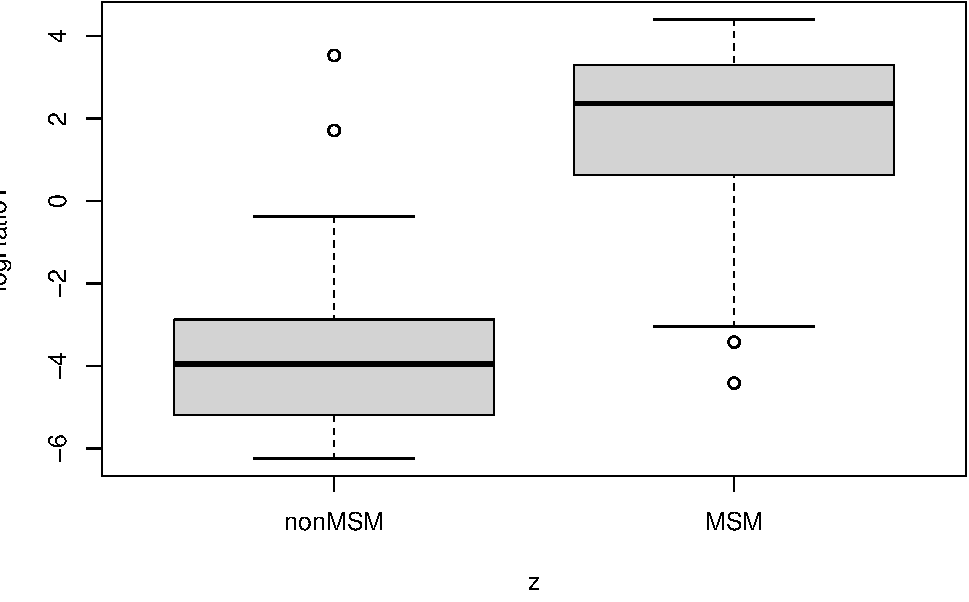
\includegraphics{guide_files/figure-latex/unnamed-chunk-22-1.pdf}

We can take things one step further and derive a second unsupervised
log-ratio biomarker, by simply fitting CoDaCoRe on the second principal
component. Taken together, our two log-ratio biomarkers capture
important information in the data:

\begin{Shaded}
\begin{Highlighting}[]
\NormalTok{pc2 }\OtherTok{=}\NormalTok{ clr }\SpecialCharTok{\%*\%}\NormalTok{ pca}\SpecialCharTok{$}\NormalTok{rotation[, }\DecValTok{2}\NormalTok{]}
\NormalTok{model }\OtherTok{\textless{}{-}} \FunctionTok{codacore}\NormalTok{(x, }\FunctionTok{as.numeric}\NormalTok{(pc2))}
\NormalTok{logRatio2 }\OtherTok{\textless{}{-}} \FunctionTok{getLogRatios}\NormalTok{(model, x)[, }\DecValTok{1}\NormalTok{]}
\FunctionTok{plot}\NormalTok{(logRatio1, logRatio2, }\AttributeTok{col =}\NormalTok{ z)}
\FunctionTok{legend}\NormalTok{(}\StringTok{"bottomleft"}\NormalTok{, }\AttributeTok{legend =} \FunctionTok{levels}\NormalTok{(z),}
    \AttributeTok{pch =} \DecValTok{1}\NormalTok{, }\AttributeTok{col =} \DecValTok{1}\SpecialCharTok{:}\DecValTok{2}\NormalTok{)}
\end{Highlighting}
\end{Shaded}

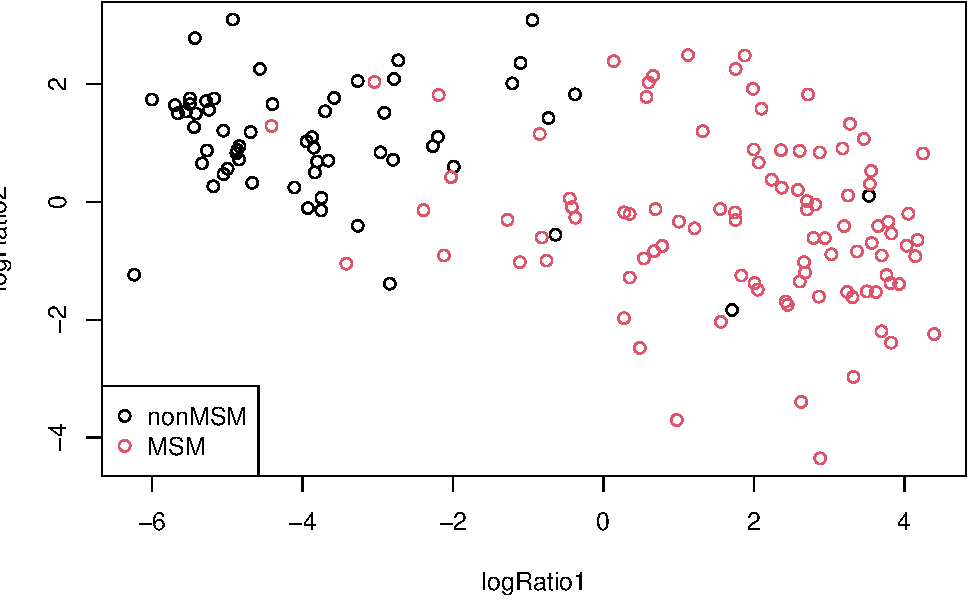
\includegraphics{guide_files/figure-latex/unnamed-chunk-23-1.pdf}

Note also that the CoDaCoRe framework can be applied to the unsupervised
learning problem in several other ways, some of which are under active
development.

\hypertarget{multi-omics-integration}{%
\section{Multi-omics integration}\label{multi-omics-integration}}

With a similar approach, CoDaCoRe can be used for scalable, sparse, and
interpretable multi-omics data integration. We briefly highlight an
example multi-omics analysis of paired gut microbiome and metabolomics
data, taken from 220 clinical samples of which 88 have Chron's disease
and 76 have ulcerative colitis
\href{https://www.nature.com/articles/s41564-018-0306-4}{(Franzosa et
al., 2019)}. For a full analysis, see Section 5 and the appendix in
\href{https://arxiv.org/abs/2104.07266}{Quinn et al., 2021}. Again, we
will use standard techniques to compute a (dense) latent representation
of the data, which we will then approximate using sparse log-ratio
biomarkers. Letting \(\mathbf T\) denote the microbe abundances
\(\mathbf U\) the metabolite abundances, we will use partial least
squares (PLS) regression to model the association between \(\mathbf T\)
and \(\mathbf U\). This will result in two latent factors, one for
\(\mathbf T\) and one for \(\mathbf U\), that capture the \emph{joint}
information in the data. These latent factors will constitute the
regression target for CoDaCoRe.

\begin{Shaded}
\begin{Highlighting}[]
\CommentTok{\# Load data}
\FunctionTok{download.file}\NormalTok{(}\StringTok{"https://github.com/egr95/FranzosaData/blob/main/FranzosaMicrobiome.rda?raw=true"}\NormalTok{,}
    \StringTok{"FranzosaMicrobiome"}\NormalTok{)}
\FunctionTok{download.file}\NormalTok{(}\StringTok{"https://github.com/egr95/FranzosaData/blob/main/FranzosaMetabolite.rda?raw=true"}\NormalTok{,}
    \StringTok{"FranzosaMetabolite"}\NormalTok{)}
\FunctionTok{load}\NormalTok{(}\StringTok{"FranzosaMicrobiome"}\NormalTok{)}
\FunctionTok{load}\NormalTok{(}\StringTok{"FranzosaMetabolite"}\NormalTok{)}

\CommentTok{\# Note data have already been}
\CommentTok{\# pre{-}processed as per (Quinn et al.,}
\CommentTok{\# 2021), including zero{-}replacement and}
\CommentTok{\# normalization to a unit total.}
\NormalTok{T }\OtherTok{\textless{}{-}}\NormalTok{ FranzosaMicrobiome[, }\SpecialCharTok{{-}}\FunctionTok{ncol}\NormalTok{(FranzosaMicrobiome)]  }\CommentTok{\# We remove the last column (response variable)}
\NormalTok{U }\OtherTok{\textless{}{-}}\NormalTok{ FranzosaMetabolite[, }\SpecialCharTok{{-}}\FunctionTok{ncol}\NormalTok{(FranzosaMetabolite)]}

\CommentTok{\# Apply clr transform prior to PLS}
\NormalTok{clrT }\OtherTok{\textless{}{-}} \FunctionTok{t}\NormalTok{(}\FunctionTok{apply}\NormalTok{(T, }\DecValTok{1}\NormalTok{, }\ControlFlowTok{function}\NormalTok{(x) }\FunctionTok{log}\NormalTok{(x) }\SpecialCharTok{{-}}
    \FunctionTok{mean}\NormalTok{(}\FunctionTok{log}\NormalTok{(x))))}
\NormalTok{clrU }\OtherTok{\textless{}{-}} \FunctionTok{t}\NormalTok{(}\FunctionTok{apply}\NormalTok{(U, }\DecValTok{1}\NormalTok{, }\ControlFlowTok{function}\NormalTok{(x) }\FunctionTok{log}\NormalTok{(x) }\SpecialCharTok{{-}}
    \FunctionTok{mean}\NormalTok{(}\FunctionTok{log}\NormalTok{(x))))}

\CommentTok{\# Call mixOmics package and plot first}
\CommentTok{\# PLS components}
\FunctionTok{suppressMessages}\NormalTok{(}\FunctionTok{library}\NormalTok{(}\StringTok{"mixOmics"}\NormalTok{))}
\NormalTok{pls }\OtherTok{\textless{}{-}}\NormalTok{ mixOmics}\SpecialCharTok{::}\FunctionTok{pls}\NormalTok{(}\AttributeTok{X =}\NormalTok{ clrT, }\AttributeTok{Y =}\NormalTok{ clrU,}
    \AttributeTok{ncomp =} \DecValTok{1}\NormalTok{)}
\FunctionTok{plot}\NormalTok{(pls}\SpecialCharTok{$}\NormalTok{variates}\SpecialCharTok{$}\NormalTok{X[, }\DecValTok{1}\NormalTok{], pls}\SpecialCharTok{$}\NormalTok{variates}\SpecialCharTok{$}\NormalTok{Y[,}
    \DecValTok{1}\NormalTok{], }\AttributeTok{main =} \StringTok{"PLS multi{-}omics (dense)"}\NormalTok{)}
\end{Highlighting}
\end{Shaded}

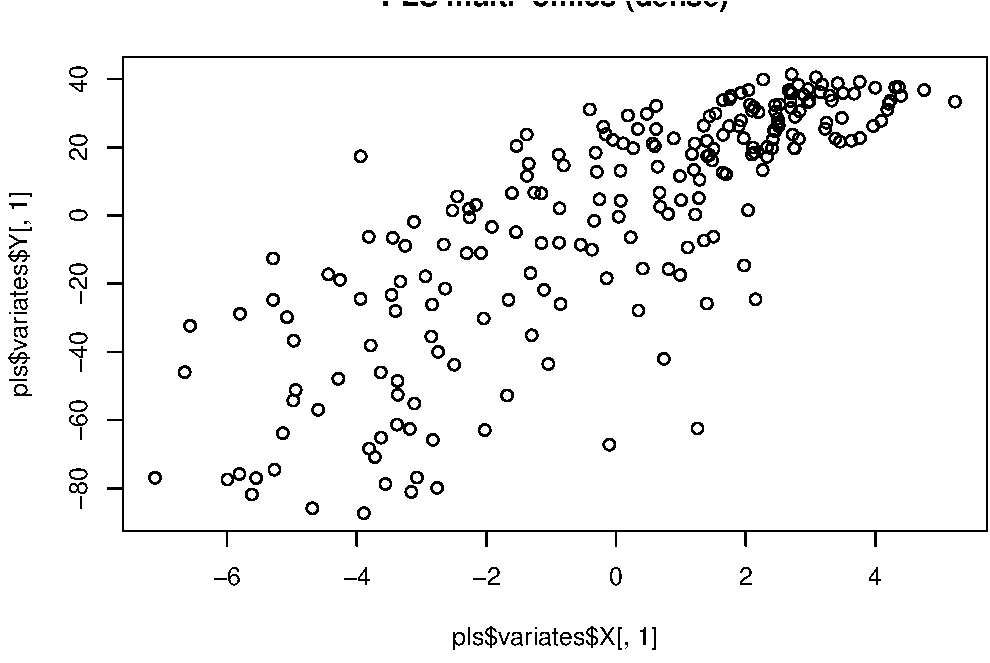
\includegraphics{guide_files/figure-latex/unnamed-chunk-24-1.pdf}

\begin{Shaded}
\begin{Highlighting}[]

\CommentTok{\# Approximate the dense PLS}
\CommentTok{\# representations with sparse log{-}ratio}
\CommentTok{\# biomarkers}
\NormalTok{plsX }\OtherTok{\textless{}{-}}\NormalTok{ pls}\SpecialCharTok{$}\NormalTok{variates}\SpecialCharTok{$}\NormalTok{X[, }\DecValTok{1}\NormalTok{]}
\NormalTok{modelX }\OtherTok{\textless{}{-}} \FunctionTok{codacore}\NormalTok{(T, plsX)}
\NormalTok{logRatioX }\OtherTok{\textless{}{-}} \FunctionTok{getLogRatios}\NormalTok{(modelX)[, }\DecValTok{1}\NormalTok{]}

\NormalTok{plsY }\OtherTok{\textless{}{-}}\NormalTok{ pls}\SpecialCharTok{$}\NormalTok{variates}\SpecialCharTok{$}\NormalTok{Y[, }\DecValTok{1}\NormalTok{]}
\NormalTok{modelY }\OtherTok{\textless{}{-}} \FunctionTok{codacore}\NormalTok{(U, plsY, }\AttributeTok{logRatioType =} \StringTok{"B"}\NormalTok{)}
\NormalTok{logRatioY }\OtherTok{\textless{}{-}} \FunctionTok{getLogRatios}\NormalTok{(modelY)[, }\DecValTok{1}\NormalTok{]}

\FunctionTok{plot}\NormalTok{(logRatioX, logRatioY, }\AttributeTok{main =} \StringTok{"CoDaCoRe multi{-}omics (sparse)"}\NormalTok{)}
\end{Highlighting}
\end{Shaded}

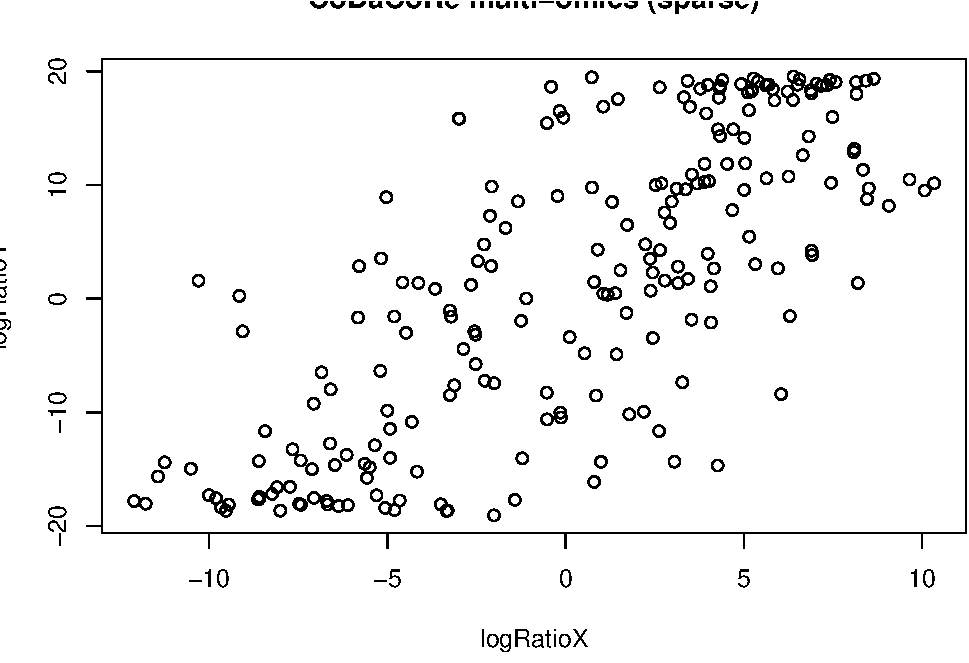
\includegraphics{guide_files/figure-latex/unnamed-chunk-24-2.pdf}

Note that CoDaCoRe obtains a sparse representation that also has better
statistical properties than the original (dense) PLS components,
markedly de-skewing the data.

\end{document}
